%*******************************************************************************
% Title: Ontoqa, Q&A with ontology-based natural language processing
%
% Conference: Courseworks in Artificial Intelligence
%
% Author: Antonella Botte <abotte@acm.org>
% Author: Giacomo Marciani <gmarciani@acm.org>
% Author: Debora Partigianoni <dpartigianoni@acm.org>
%
% Institution: Department of Civil Engineering and Computer Science Engineering,
%         University of Rome Tor Vergata, Italy
%
% Style: ACM Large VERSION 2017
%*******************************************************************************

\documentclass[acmlarge]{acmart}

%*******************************************************************************
% Packages
%*******************************************************************************
\usepackage[utf8]{inputenc}
\usepackage{amsmath}
\usepackage{booktabs}
\usepackage{lipsum}
\usepackage{caption}
\usepackage{array}
\usepackage{xr}
\usepackage{tikz}
\usepackage{tikz-qtree}
\usetikzlibrary{positioning}
\usepackage[ruled,noend,noline]{algorithm2e}

%*******************************************************************************
% Meta
%*******************************************************************************
\acmJournal{ACMROME-CP}
\acmVolume{1}
\acmNumber{1}
\acmArticle{1}
\acmYear{2017}
\acmMonth{2}
\acmArticleSeq{11}
\acmDOI{0000001.0000001}
\acmPrice{0.00}
\received[accepted]{May 2017}

%*******************************************************************************
% Copyright
%*******************************************************************************
\setcopyright{rightsretained}

%*******************************************************************************
% Algorithm
%*******************************************************************************
\usepackage[ruled]{algorithm2e}
\renewcommand{\algorithmcfname}{ALGORITHM}
\SetAlFnt{\small}
\SetAlCapFnt{\small}
\SetAlCapNameFnt{\small}
\SetAlCapHSkip{0pt}
\IncMargin{-\parindent}

%*******************************************************************************
% Custom Commands
%*******************************************************************************

%*******************************************************************************
% Numbering
%*******************************************************************************
\numberwithin{equation}{section}

%*******************************************************************************
% References
%*******************************************************************************
\externaldocument{sec/introduction}
\externaldocument{sec/background}
\externaldocument{sec/architecture}
\externaldocument{sec/grammar}
\externaldocument{sec/ontology}
\externaldocument{sec/parsing}
\externaldocument{sec/implementation}
\externaldocument{sec/sample-execution}
\externaldocument{sec/evaluation}
\externaldocument{sec/improvements}
\externaldocument{sec/conclusions}

\begin{document}
%*******************************************************************************
% Title and Authors
%*******************************************************************************
\title{Ontoqa, Q\&A with ontology-based natural language processing}
\author{Antonella Botte}
\orcid{0000-0000-0000-0000}
\affiliation{%
  \institution{University of Rome Tor Vergata}
  \streetaddress{Via del Politecnico 1}
  \city{Rome}
  \state{RM}
  \postcode{00133}
  \country{IT}}
\author{Giacomo Marciani}
\orcid{0000-0002-3675-8804}
\affiliation{%
  \institution{University of Rome Tor Vergata}
  \streetaddress{Via del Politecnico 1}
  \city{Rome}
  \state{RM}
  \postcode{00133}
  \country{IT}}
\author{Debora Partigianoni}
\orcid{0000-0000-0000-0000}
\affiliation{%
  \institution{University of Rome Tor Vergata}
  \streetaddress{Via del Politecnico 1}
  \city{Rome}
  \state{RM}
  \postcode{00133}
  \country{IT}}

%*******************************************************************************
% Front
%*******************************************************************************
\begin{abstract}
	
% MOTIVATION
Natural language processing (NLP) is a family of technologies that can disruptively reshape human-machine interaction, data-driven decision making and daily exploration of knowledge by humans.
%
One of the most representative and widely studied NLP application is question-answering (Q\&A).
%
With the fast growing diffusion of semantic web and advancement in NLP technologies, Q\&A systems will be one of the most important interface to knowledge.


% PROBLEM STATEMENT
Since it is not possible to develop a single ontology to effectively capture the whole knowledge, it is necessary to develop Q\&A systems that can easily adapt to distinct ontologies and lexicons.


% APPROACH
In this work we describe Ontoqa, a Q\&A web and standalone application which aims to achieve this ambitious goal.
%
The proposed solution leverages ontology-driven NLP through the use of the LTAG/DUDES model and a greedy parsing algorithm aiming to reduce both the syntactic and semantic search space.
%
%
% RESULTS
The experimental results show that our system can answer the benchmark questions, with good performance with respect to both response-time and memory usage. 
%
%
% CONCLUSIONS
Our work shows that ontology alignment through the LTAG/DUDES model permits 
high modularization and generalization of the NLP process.
%
Furthermore, such a model suits well to the design of parsing algorithms that can effectively minimize both the syntactic and semantic search space.
 

\end{abstract}

% http://dl.acm.org/ccs.cfm

\begin{CCSXML}
    <ccs2012>
    <concept>
        <concept_id>10002944.10011122.10002945</concept_id>
        <concept_desc>General and entry~Surveys and overviews</concept_desc>
        <concept_significance>500</concept_significance>
    </concept>
    <concept>
        <concept_id>10002978</concept_id>
        <concept_desc>Security and privacy</concept_desc>
        <concept_significance>500</concept_significance>
    </concept>
    <concept>
        <concept_id>10002978.10003022</concept_id>
        <concept_desc>Security and privacy~Software and application security</concept_desc>
        <concept_significance>500</concept_significance>
    </concept>
    </ccs2012>
\end{CCSXML}

\ccsdesc[500]{General and entry~Surveys and overviews}
\ccsdesc[500]{Security and privacy~Software and application security}

\keywords{computer security; botnet}


%*******************************************************************************
% Thanks
%*******************************************************************************
\thanks{
  This work is supported by the Department of Civil Engineering and Computer Science
  Engineering, University of Rome Tor Vergata, Italy.\\
  Author's address:
  A. Botte, Via del Politecnico 1, Rome, RM 00133, Italy;
  email: abotte@acm.org;
  G. Marciani, Via del Politecnico 1, Rome, RM 00133, Italy;
  email: gmarciani@acm.org;
  D. Partigianoni, Via del Politecnico 1, Rome, RM 00133, Italy;
  email: dpartigianoni@acm.org;
}

\maketitle

\renewcommand{\shortauthors}{A. Botte, G. Marciani and D. Partigianoni}

%*******************************************************************************
% Core Content
%*******************************************************************************
\section{Introduction}
\label{sec:introduction}

% CONTEXT: NLP and QA
Natural Language Processing (NLP) is a theoretically motivated range of
computational techniques for analyzing and representing naturally occurring texts
at one or more levels of linguistic analysis for the purpose of achieving human-like
language processing for a range of tasks or applications \cite{liddy2001natural}.

NLP can disruptively reshape human-machine interaction, data-driven decision-making and daily exploration of knowledge by humans.
%
One of the most representative and widely studied NLP application is question-answering (Q\&A).
%
With the fast growing diffusion of semantic web and advancement in NLP technologies, Q\&A systems will be one of the most important interface to knowledge.

% CHALLENGE
It is well-known that it is not possible to develop a single ontology to effectively capture the whole knowledge.
%
This theoretical and intuitive limit makes necessary to develop Q\&A systems that can easily adapt to distinct ontologies and lexicons.
%
This theoretical and intuitive limit makes necessary to develop Q\&A systems that can easily adapt to distinct ontologies and lexicons.

% GOAL
The goal of the presented research is to address this  challenge.
%
In this work we describe \textit{Ontoqa}, a Q\&A web and standalone application which aims to achieve this ambitious goal.
%
The proposed solution leverages (i) ontology-driven NLP through the use of the LTAG/DUDES model and (ii) a parsing algorithm that aims to reduce both the syntactic and  semantic search space \cite{cimiano2014ontology}.


% REMAINDER
The remainder of the paper is organized as follows:
Section~\ref{sec:background} gives the background context, useful to better understand our work;
Section~\ref{sec:architecture} shows the architecture implemented in our solution;
Section~\ref{sec:grammar} shows the grammar used to parse the natural language;
Section~\ref{sec:ontology} shows the ontology used to semantically represent the reference domain;
Section~\ref{sec:parsing} shows the algorithm used for question parsing;
Section~\ref{sec:implementation} shows how the application has been implemented, with a focus on the adopted technologies;
Section~\ref{sec:evaluation} shows the experiemntal results, focusing on both response time and memory usage;
Section~\ref{sec:sample-execution} shows some representative parsing executions on benchmark questions;
Section~\ref{sec:further-improvements} outlines the possible improvements for the proposed work;
Section~\ref{sec:conclusions} concludes this article, summarizing our work and results.
\section{Background}
\label{sec:background}
% ANTONELLA
The context in which this work lies is the ontology-based interpretation of natural language. This approach puts ontology at the center of the interpretative process and assumes that for each ontology there are several lexicons, so this technique requires an expert to generate the specific lexicon for that ontology and domain.

Another aspect of this approach is the grammar used by the system for the interpretation of natural language in the context of a given ontology. These grammars are based on a vocabulary aligned with ontology and contain syntactic and semantic information that are crucial to the compositional process of the meaning of the sentence with respect to the precise ontology.
Domain-specific grammars are then used together with other domain-independent grammars, such as pronouns and auxiliary verbs.

%
This approach combines the ultimate purpose of the system realized as such tools will be used to build a question-answering system, where natural language application is transformed into a formal query through a linguistic analysis that is guided by the grammar ontology-based.
Formally, the three key aspects are defined:\textbf{Ontology}, \textbf{Grammar}, \textbf{Ontology Lexica}.

\subsection{Ontology}
\theoremstyle{definition}
\begin{definition}
\newtheorem{defn}{Definition}[section]{\textbf{Ontology}.Given a conceptualization \textit{C},an ontology \textit{O} is a logical theory with an ontological commitment  \textit{K} such that the models of the logical theory approximate as well as possible the set of intended models \begin{math}I_k(O)\end{math}}
\end{definition}

\subsection{Ontology Lexica}

\textit{Ontology lexica} (Cimiano et al., 2007; Peters et al., 2007) specify how words, phrases etc. should
be interpreted in the context of a given domain ontology
and are thus crucial for ontology-based NLP applications \cite{mccrae2012three} .

The Lexicon Model for Ontologies, or lemon for short, is such a model for specifying the lexicon-ontology interface, allowing one to state the meaning of lexical entries and constructions with respect to the vocabulary of a given ontology declaratively.

The lemon model follows a principle that has been referred to as semantics by reference and states that the meaning of a lexical entry is specified by reference to a certain ontological class, property or individual.

The LexInfo ontology extends the lemon model with more than 600 specific linguistic categories.It can be used to add properties to different forms of a lexical entry. LexInfo is an ontology and thusallows for consistency checking and reasoning. 

In general, each lexical entry in a lemon lexicon has a number of syntactic arguments that map to semantic arguments of an ontological property or a more complex semantic frame. In general, we require that there is a one-to-one mapping between syntactic arguments subcategorized by a certain lexical entry and the set of semantic arguments specified in the lexical entry. For all lexical entries, we assume that there is a stereotypical usage or construction involving the lexical entry in which all syntactic arguments are actually realized.

\subsection{Grammar}
The grammar consists of syntactic and semantic part:
\begin{itemize} 
  \item Syntax studies how words are combined into phrases and sentences
  \item Semantics investigates the meanings of expressions of a language, and how the meanings of basic expressions are combined into meanings of more complex expressions
\end{itemize} 
There are two particular formalisms for the representation of the semantics and syntax of a sentence.

%LTAG
The syntactic part is represented by LTAG( Lexicalized Tree Adjoining Grammar).  
The Tree Adjoining Grammar (TAG) is a linguistic formalism that builds trees as representations of syntactic structure, and the TAG's fundamental hypothesis is that every syntactic dependency is expressed locally within a single elementary tree. Lexicalized grammars assume that each atomic element or structure is associated with a lexical item. With respect to TAG, this means that elementary trees have to be associated with at least one lexical element, i.e., contains at least one leaf node labled with a non-empty terminal symbol.

%DUDES
For semantic representation, we speak of representation DUDES (Dependency-based Underspecified Discourse Representation Structures).
A DUDES is a triple  \textit{(v,D,S)} where 
\begin{itemize} 
  \item  \textit{S} \begin{math}\epsilon \end{math} \textit{U} is a referent marker (the distinguished or main variable),
  \item \textit{D}=\textit{(U,C)} is a DRS with a discourse universe U and a set of conditions C, 
  \item  \textit{S} is a set of selection pairs of the form (N,v) where N is a LTAG tree node label and v is
a referent marker.
\end{itemize} 
\section{Architecture}
\label{sec:architecture}
% ANTONELLA
The system created allows the user to enter a question in natural language, this question the system intends to translate it into a formal query through the ontology-based grammar-based language analysis and to which ontology answers in Based on the content of the application.
\begin{itemize}
	\item Grammar generation
	\item Linguistic analysis of demand and answer to the user
\end{itemize}

\subsection{Grammar generator}
Grammar has been assumed made up of two parts: one depending on ontology, and another independent. The domain specific grammar refers to the part that contains the lexical entries like individuals, concepts and properties contained in the ontology. The ontological independent part contains expressions like auxiliary verbs, determiners, wh-words, and so on.

Generally what he does is represented as follows:

\begin{figure}[H]
   \centering
    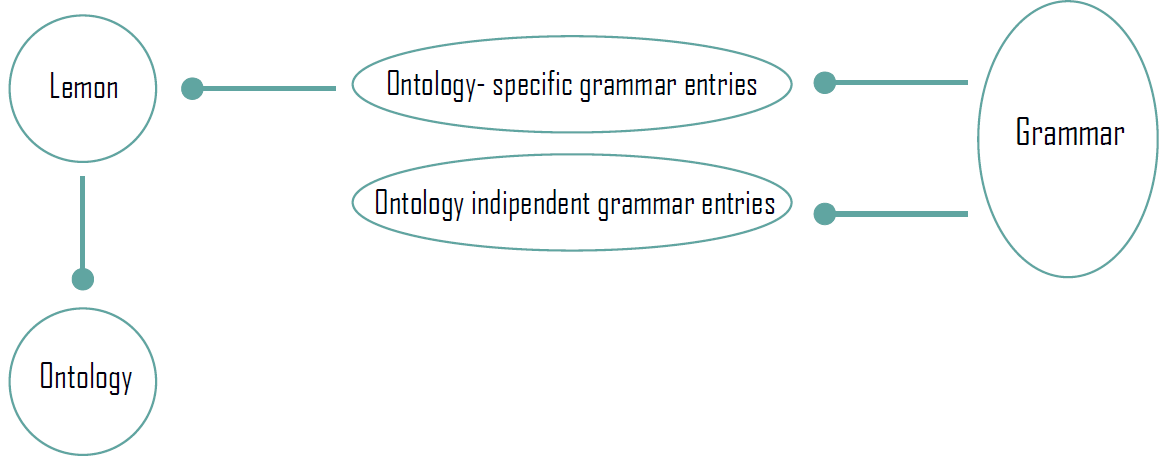
\includegraphics[scale=0.5]{./fig/grammar}
    \label{fig:grammar}
    \caption{The Grammar.}
\end{figure}

Both parts of the grammar use the main linguistic representations or each grammar is represented as a pair of syntactic and semantic representations. As a syntactic representation, Lexicalized Tree Adjoining Grammar (LTAG) is used. As semantic representations we take Dudes.

The first step in generating a grammar from a given ontology is to enrich the ontology with information about its verbalization. To achieve this we leaverage LexInfo, which uses a general frame to create a declarative specification of the lexicon-ontology interface by connecting concepts of the ontology to information about their linguistic realization, i.e. word forms, morphology, sub-categoriziation frames and how syntactic and semantic arguments correspond to each other. The lexical entries specified by LexInfo are then used to generate grammar entries, i.e. indexed LTAG/DUDES.

\subsection{Ontoqa}
The system provides the user with an intuitive interface to submit questions, expressed in English natural language.

The natural language question is processed by the parser to generate the corresponding LTAG/DUDES representation, from which a formal SPARQL query can be obtained.
%After the disambiguation and obtaining of the SLTAG of our universe of speech, we generate a formal query. The formal query will be submitted to the ontology that will return us an answer. 
Finally, the query is submitted to the ontology, thus retrieving the output answer.
The procedure is shown in the Figure.

%The system allows a user to submit, via an intuitive interface, a natural-language question in English.

%Given the question in Natural Language, a parsing is applied that constructs an LTAG derivative tree considering only the syntactic part of the grammatical voices involved.

%Subsequently, syntactic and semantic composition rules apply to the construction of a tree in accordance with the LTAG derivation tree and DUDES semantics.

%In general, what happens is that LTAG provides substitution and adjunction rules while DUDES semantics provides rules as saturation operations that are interpreted as substitutions and a union operation that interprets the adjoin.



\begin{figure}[H]
   \centering
    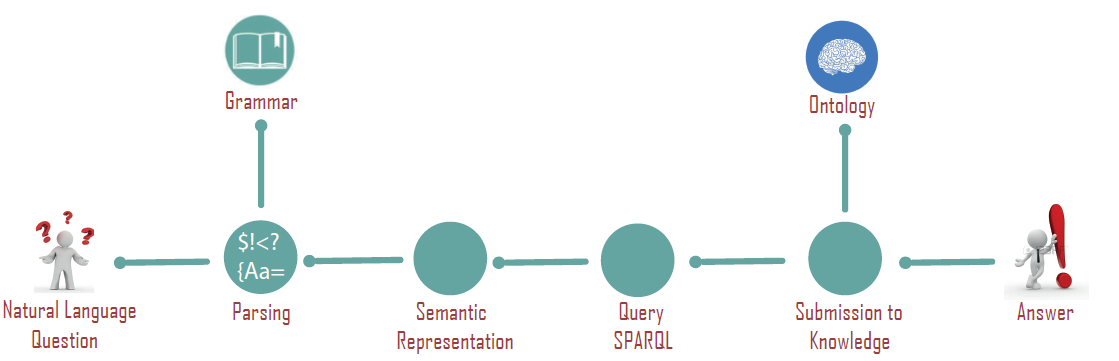
\includegraphics[scale=0.5]{./fig/ontoqa}
    \label{fig:ontoqa}
    \caption{The workflow.}
\end{figure}
\section{Grammar}
\label{sec:grammar}

% ANTONELLA E DEBORA
The LTAG/DUDES grammars consists of two parts: a domain-specific one obtained by extracting all relevant information from the ontology lexicon, and a domain-independent one created manually comprising closed-class expressions such as determiners, pronouns, copulative and auxiliary verbs.

It is important to note that the grammar entries are indexed with regular-expressions. So the grammar entries can be composed not only by a single word but also by a more complex expression. The reader can refer to the Section~\ref{sec:parsing} for details on matching the specified entry in english natural language with the entries of LTAG/DUDES in the grammar.

\subsection{DOMAIN-SPECIFIC GRAMMAR}
Talking about the automatic generation of domain-specific grammar, we have created one LTAG/DUDES for each lexicon entry and for all its different forms. The types of lexicon entry we addressed are: \textit{verbs, common nouns, proper nouns, prepositions and adjectives}.

\subsubsection{VERBS}\mbox{}\\
All the verbs we need in the ontology lexicon in \textit{lemon} format are transitive verbs with active voice and indicative mood. The tree and the semantic representation would thus look as follows:

\medskip
\begin{center}
	\captionof{figure}{Grammar entry for: "acquire"}
\begin{tabular}{ p{10em} p{10em} }
	\label{tbl:grammar.acquire}
	
	\begin{center}
		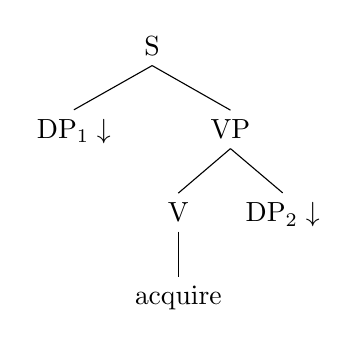
\begin{tikzpicture}
		\Tree [.S [.DP$_1\downarrow$ ] [.VP [.V acquire ] DP$_2\downarrow$ ] ]	
		\end{tikzpicture}
	\end{center}
	
	&

	\begin{center}
		\begin{tabular}{|c|l|}
			\hline
			\mbox{} & \mbox{}\\
			\hline
			\multicolumn{2}{|l|}{
				$isAcquiredBy(x,y)$
			} \\
			\hline
			\multicolumn{2}{|l|}{
				$(y,DP_{1}),(x,DP_{2})$
			} \\
			\hline
		\end{tabular}
	\end{center}	
	\\
\end{tabular}
\end{center}
\medskip

\subsubsection{NOUNS}\mbox{}\\
We can distinguish between common nouns, relational nouns and proper nouns. If the lexical entry of the ontology lexicon in \textit{lemon} has the syntactic argument \textit{possessiveAdjunct} we have a \textbf{relational noun} and the elementary LTAG/DUDES would thus look as follows: 

\medskip
\begin{center}
	\captionof{figure}{Grammar entry for: "chairman of"}
\begin{tabular}{ p{10em} p{10em} }
	\label{tbl:grammar.chairmanOf}
	
	\begin{center}
		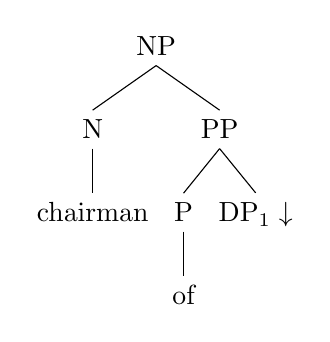
\begin{tikzpicture}
		\Tree [.NP [.N chairman ] [.PP [.P of ] DP$_1\downarrow$ ] ]
		\end{tikzpicture}
	\end{center}
		
	&
	
	\begin{center}
		\begin{tabular}{|c|l|}
			\hline
			y & \mbox{}\\ 
			\hline
			\multicolumn{2}{|l|}{
				$hasChairman(x,y)$
			} \\
			\hline
			\multicolumn{2}{|l|}{
				$(x,DP_{1})$
			} \\
			\hline
		\end{tabular}
	\end{center}	
	\\
\end{tabular}
\end{center}
\medskip

Simple common nouns and proper nouns differ from relational nouns in their syntactic behavior and sense. A \textbf{common noun}, as \textit{CEO, corporate officer}, and so on, has the following elementary LTAG/DUDES:

\medskip
\begin{center}
	\captionof{figure}{Grammar entry for: "people"}
\begin{tabular}{ p{10em} p{10em} }
	\label{tbl:grammar.people}
	
	\begin{center}
		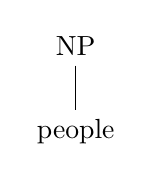
\begin{tikzpicture}
		\Tree [.NP people ]
		\end{tikzpicture}
	\end{center}
		
	&
	
	\begin{center}
		\begin{tabular}{|c|l|}
			\hline
			x & \mbox{}\\ 
			\hline
			\multicolumn{2}{|l|}{
				$Person(x)$
			} \\
			\hline
			\multicolumn{2}{|l|}{
				\mbox{}
			} \\
			\hline
		\end{tabular}
	\end{center}	
	\\
\end{tabular}
\end{center}
\medskip

A \textbf{proper noun}, e.g. \textit{Microsoft}, has instead the following elementary LTAG/DUDES:
 
\medskip
\begin{center}
	\captionof{figure}{Grammar entry for: "Microsoft"}
\begin{tabular}{ p{10em} p{10em} }
	\label{tbl:grammar.microsoft}
	
	\begin{center}
		
\begin{tikzpicture}
		\Tree [.DP Microsoft ]
		\end{tikzpicture}
	\end{center}
		
	&
	
	\begin{center}
		\begin{tabular}{|c|l|}
			\hline
			x & x\\ 
			\hline
			\multicolumn{2}{|l|}{
				$x=Microsoft$
			} \\

			\hline
			\multicolumn{2}{|l|}{
				\mbox{}
			} \\
			\hline
		\end{tabular}
	\end{center}	
	\\
\end{tabular}
\end{center}
\medskip

\subsubsection{ADJECTIVES}\mbox{}\\
We have different types of adjectives. Let's take some examples:
\begin{enumerate}
\item "\textit{an \textbf{italian} company}". In this case \textit{italian} is an \textbf{attributive} adjective and the associated grammar is the following:
 \medskip
\begin{center}
	\captionof{figure}{Grammar entry for: "italian" - attributive adjective}
\begin{tabular}{ p{10em} p{10em} p{10em} }
	\label{tbl:grammar.attributiveAdjective}
	
	\begin{center}
		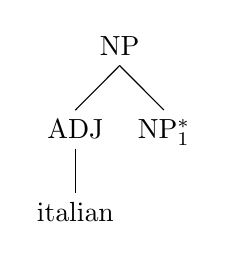
\begin{tikzpicture}
		\Tree [.NP [.ADJ italian ] [.NP$_1^\ast$ ] ]
		\end{tikzpicture}
	\end{center}
		
	&
	
	\begin{center}
		\begin{tabular}{|c|l|}
			\hline
			x & \mbox{}\\ 
			\hline
			\multicolumn{2}{|l|}{
				$hasNationality(x,y)$
			} \\
			\multicolumn{2}{|l|}{
				$y=Italy$
			} \\
			\hline
			\multicolumn{2}{|l|}{
				\mbox{}
			} \\
			\hline
		\end{tabular}
	\end{center}	
	
	&
	
	\begin{center}
		\begin{tabular}{|c|l|}
			\hline
			x & \mbox{}\\ 
			\hline
			\multicolumn{2}{|l|}{
				$hasHeadquarter(x,y)$
			} \\
			\multicolumn{2}{|l|}{
				$y=Italy$
			} \\
			\hline
			\multicolumn{2}{|l|}{
				\mbox{}
			} \\
			\hline
		\end{tabular}
	\end{center}	
	\\
\end{tabular}
\end{center}
\medskip
To note that \textit{italian} and similar adjectives are ambiguous in the lexicon. For more details on dealing with ambiguities, refer to Section~\ref{sec:parsing}.
\item "\textit{Is Satya Nadella \textbf{italian}?}". In this example \textit{italian} is a  \textbf{predicative} adjective and the elementary LTAG/DUDES are:
\medskip
\begin{center}
	\captionof{figure}{Grammar entry for: "italian" - predicative adjective}
\begin{tabular}{ p{10em} p{10em} p{10em}}
	\label{tbl:grammar.predicativeAdjective}
	
	\begin{center}
		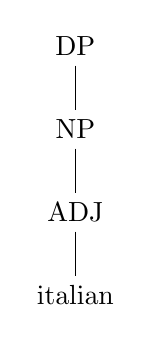
\begin{tikzpicture}
		\Tree [.DP  [.NP [.ADJ italian ] ] ]
		\end{tikzpicture}
	\end{center}
		
	&

	\begin{center}
		\begin{tabular}{|c|l|}
			\hline
			\mbox{x} & x y \\
			\hline
			\multicolumn{2}{|l|}{
				$hasNationality(x,y)$
			} \\
			\multicolumn{2}{|l|}{
				$y=Italy$
			} \\
			\hline
			\multicolumn{2}{|l|}{
				\mbox{}
			} \\
			\hline
		\end{tabular}
	\end{center}
	
	&
	
	\begin{center}
		\begin{tabular}{|c|l|}
			\hline
			\mbox{x} & x y \\
			\hline
			\multicolumn{2}{|l|}{
				$hasHeadquarter(x,y)$
			} \\
			\multicolumn{2}{|l|}{
				$y=Italy$
			} \\
			\hline
			\multicolumn{2}{|l|}{
				\mbox{}
			} \\
			\hline
		\end{tabular}
	\end{center}
	\end{tabular}
\end{center}
\medskip
\item "\textit{headquartered in Italy}". In this third case \textit{headquarters} is a \textbf{prepositional} adjective. The grammar is the following:

\medskip
\begin{center}
	\captionof{figure}{Grammar entry for: "headquartered in"}
\begin{tabular}{ p{10em} p{10em} }
	\label{tbl:grammar.headquarteredIn}
	
	\begin{center}
		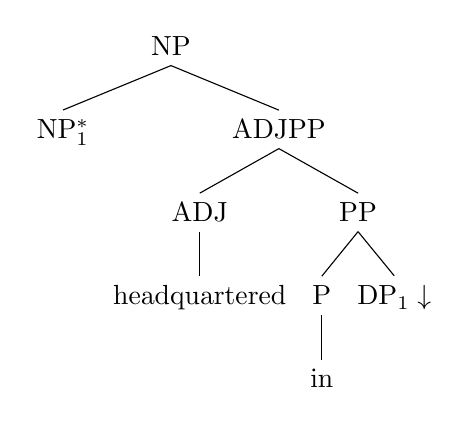
\begin{tikzpicture}
		\Tree [.NP [.NP$_1^\ast$ ] [.ADJPP [.ADJ headquartered ] [.PP [.P in ] DP$_1\downarrow$ ] ] ]	
		\end{tikzpicture}
	\end{center}
	
	&

	\begin{center}
		\begin{tabular}{|c|l|}
			\hline
			x & \mbox{}\\
			\hline
			\multicolumn{2}{|l|}{
				$hasHeadquarter(x,y)$
			} \\
			\hline
			\multicolumn{2}{|l|}{
				$(y,DP_{1})$
			} \\
			\hline
		\end{tabular}
	\end{center}	
	\\
\end{tabular}
\end{center}
\medskip
\item "\textit{Where is Microsoft headquartered?}". For adjectives as \textit{headquartered} the grammar contains a further entry composed by the regular expression "\textit{is * headquartered}". The "*" can represent any expression and this regular expression generates the following grammar:
\medskip
\begin{center}
	\captionof{figure}{Grammar entry for: "is * headquartered"}
\begin{tabular}{ p{10em} p{10em} }
	\label{tbl:grammar.is*headquartered}
	
	\begin{center}
		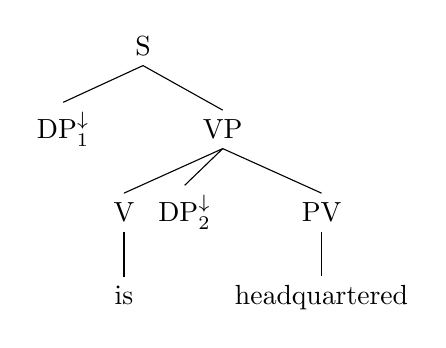
\begin{tikzpicture}
		\Tree [.S [.DP$_1^\downarrow$ ] [.VP [.V is ] DP$_2^\downarrow$ [.PV headquartered ] ] ]	
		\end{tikzpicture}
	\end{center}
	
	&

	\begin{center}
		\begin{tabular}{|c|l|}
			\hline
			\mbox{} & \mbox{}\\
			\hline
			\multicolumn{2}{|l|}{
				$hasHeadquarter(x,y)$
			} \\
			\hline
			\multicolumn{2}{|l|}{
				$(x, DP_{2}),(y,DP_{1})$
			} \\
			\hline
		\end{tabular}
	\end{center}	
	\\
\end{tabular}
\end{center}
\medskip
\end{enumerate}


\subsection{DOMAIN-INDEPENDENT GRAMMAR}
For the domain-independent expressions, we generate manually a fixed grammar entry for each word or expression we could encounter. For example there is a grammar for the expression \textit{how many}:
 \medskip
\begin{center}
	\captionof{figure}{Grammar entry for: "How many"}
\begin{tabular}{ p{10em} p{10em} }
	\label{tbl:grammar.howMany}
	
	\begin{center}
		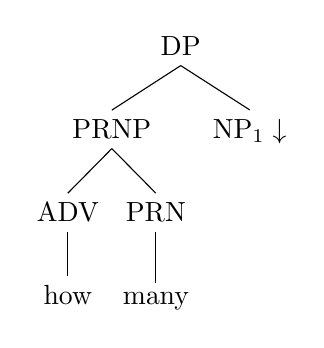
\begin{tikzpicture}
		\Tree [.DP  [.PRNP [.ADV how ] [.PRN many ]] [.NP$_1\downarrow$ ]]
		\end{tikzpicture}
	\end{center}
		
	&
	
	\begin{center}
		\begin{tabular}{|c|l|}
			\hline
			x & x\\ 
			\hline
			\multicolumn{2}{|l|}{
				$count(x)$
			} \\
			\hline
			\multicolumn{2}{|l|}{
				$(x,NP_{1})$
			} \\
			\hline
		\end{tabular}
	\end{center}	
	\\
\end{tabular}
\end{center}
\medskip

The auxiliary verbs, as \textit{do, does, did, have, has, had}, don't have a semantic interpretation, so the DUDES is empty. The elementary LTAG instead is in the form of adjunction tree:
\medskip
\begin{center}
	\captionof{figure}{Grammar entry for: "do"}
\begin{tabular}{ p{10em} p{10em} }
	\label{tbl:grammar.do}
	
	\begin{center}
		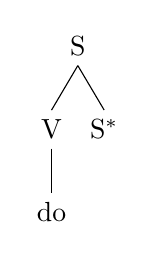
\begin{tikzpicture}
		\Tree [.S  [.V do ] [.S$^\ast$ ]]
		\end{tikzpicture}
	\end{center}
	&
	\begin{center}
		\begin{tabular}{|c|l|}
			\hline
			\mbox{} & \mbox{}\\ 
			\hline
			\multicolumn{2}{|l|}{
				\mbox{}
			} \\
			\hline
			\multicolumn{2}{|l|}{
				\mbox{}
			} \\
			\hline
		\end{tabular}
	\end{center}	
	\\
\end{tabular}
\end{center}
\medskip

We have generated grammar also for determiners, pronouns and copulative verbs. Determiners, i.e. \textit{the, a, an} has the following elementary LTAG/DUDES:
\medskip
\begin{center}
	\captionof{figure}{Grammar entry for: "the"}
\begin{tabular}{ p{10em} p{10em} }
	\label{tbl:grammar.the}
	
	\begin{center}
		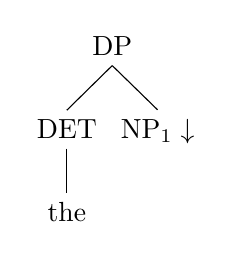
\begin{tikzpicture}
		\Tree [.DP  [.DET the ] [.NP$_1\downarrow$ ]]
		\end{tikzpicture}
	\end{center}
		
	&

	\begin{center}
		\begin{tabular}{|c|l|}
			\hline
			x & x\\ 
			\hline
			\multicolumn{2}{|l|}{
				\mbox{}
			} \\
			\hline
			\multicolumn{2}{|l|}{
				$(x,NP_{1})$
			} \\
			\hline
		\end{tabular}
	\end{center}	
	\\
\end{tabular}
\end{center}
\medskip

The grammar of wh-pronoun, as \textit{who, what, where, which}, is:
\medskip
\begin{center}
	\captionof{figure}{Grammar entry for: "who"}
\begin{tabular}{ p{10em} p{10em} }
	\label{tbl:grammar.who}
	
	\begin{center}
		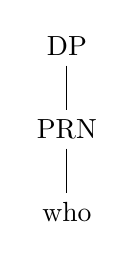
\begin{tikzpicture}
		\Tree [.DP  [.PRN who ] ]
		\end{tikzpicture}
	\end{center}
		
	&

	\begin{center}
		\begin{tabular}{|c|l|}
			\hline
			x & ?x\\ 
			\hline
			\multicolumn{2}{|l|}{
				\mbox{}
			} \\
			\hline
			\multicolumn{2}{|l|}{
				\mbox{}
			} \\
			\hline
		\end{tabular}
	\end{center}	
	\\
\end{tabular}
\end{center}
\medskip

Finally, we have to considered the copulative verbs. They have two different syntactic representations, for example consider the following questions:
\begin{enumerate}
\item \textit{Where is Microsoft headquartered?}
\item \textit{Is Satya Nadella the CEO of Microsoft?}
\end{enumerate}
In the first case, the copulative verb \textit{is} has the grammar :
\medskip
\begin{center}
	\captionof{figure}{Grammar entry for: "is" (1)}
\begin{tabular}{ p{10em} p{10em} }
	\label{tbl:grammar.is}
	
	\begin{center}
		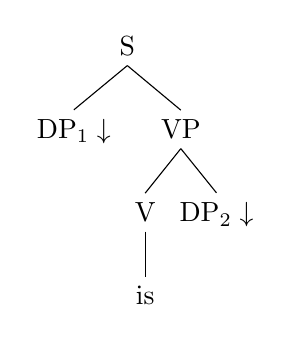
\begin{tikzpicture}
		\Tree [.S [.DP$_1\downarrow$ ] [.VP [.V is ] DP$_2\downarrow$ ] ]	
		\end{tikzpicture}
	\end{center}
	
	&

	\begin{center}
		\begin{tabular}{|c|l|}
			\hline
			\mbox{} & \mbox{}\\
			\hline
			\multicolumn{2}{|l|}{
				$replace(y,x)$
			} \\
			\hline
			\multicolumn{2}{|l|}{
				$(x,DP_{1}),(y,DP_{2})$
			} \\
			\hline
		\end{tabular}
	\end{center}	
	\\
\end{tabular}
\end{center}
\medskip

In the second case the grammar have to be the following:
\medskip
\begin{center}
	\captionof{figure}{Grammar entry for: "is" (2)}
\begin{tabular}{ p{10em} p{10em} }
	\label{tbl:grammar.is}
	
	\begin{center}
		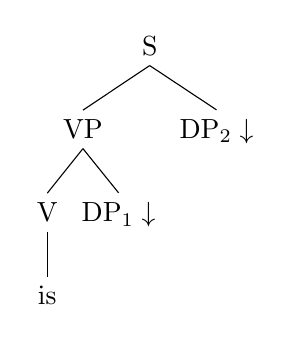
\begin{tikzpicture}
		\Tree [.S [.VP [.V is ] DP$_1\downarrow$ ] [.DP$_2\downarrow$ ] ]	
		\end{tikzpicture}
	\end{center}
	
	&

	\begin{center}
		\begin{tabular}{|c|l|}
			\hline
			\mbox{} & \mbox{}\\
			\hline
			\multicolumn{2}{|l|}{
				$replace(y,x)$
			} \\
			\hline
			\multicolumn{2}{|l|}{
				$(x,DP_{1}),(y,DP_{2})$
			} \\
			\hline
		\end{tabular}
	\end{center}	
	\\
\end{tabular}
\end{center}
\medskip
\section{Ontology}
\label{sec:ontology}
% DEBORA
The domain chosen for our ontology is "Organizations". The domain ontology expresses the links between specific objects and events of that domain through classes (or concepts), properties and attributes of the classes, constraints and instances. The ontology has been modelled to answer the benchmark questions, though it is not strictly limited to them.
The concepts we want to represent are:
\begin{itemize}
\item The companies.
\item People who play an important role in the company.
\item A nation for the nationality of people or for the headquarter of a company.
\end{itemize}
The symbols we used to represent this sets are: \textit{Company, Person} and \textit{Nation}.
Then we need symbols to represent the relationships between classes. The relationships we needed are:
\begin{itemize}
\item A person who is the founder of a company.
\item A person who is the CEO of a company.
\item A person who is the CFO of a company.
\item A person who is the Chairman of a company.
\item A person who is the Corporate Officer of a company.
\item A company acquiring a company.
\item The nationality of people.
\item The nation where the headquarter of a company is located.
\end{itemize}
The symbols we used to represent these relationships are: \textit{hasFounder, hasCEO, hasCFO, hasChairman, hasCorporateOfficer, isAcquiredBy, hasNationality} and \textit{hasHeadquarter}. 

We also introduced some attribute to classes:
\begin{itemize}
\item The net income of an organization.
\item The market value of a company. For multinational company the market value is referred to the market capitalization. For smaller companies, subsidiaries whose business operations and investments are controlled by the parent corporation, the market value is referred to value at which a company is acquired.
\end{itemize}
The symbols we used to represent these attributes are: \textit{ netIncome} and \textit{marketValue}.
Both the net income and the purchase price are in \textit{billion U.S. dollars}. To note that a billion, in American English, has always equated to a thousand million (i.e. 1'000'000'000).

In order to prevent a computer program to use the symbols '\textit{in the wrong way}' we have introduced  constraints on the way the vocabulary is used:
\begin{itemize}
\item a person can not be a company and a company can not be a person.
\item people must have at least one nationality.
\item companies must have at least one headquarter. 
\end{itemize}

The reader can refer to the files \textit{organizationVersion2.ttl} in the \textit{data/knowledge} package and \textit{organizationNotInfVersion2.ttl} in \textit{data/knowledge/protégé} to see the ontology in detail. The first file is obtained merging the inferred and asserted information of our ontology. The second one contains only the asserted informations.  

At the \textit{data/knowledge} path there is also the first version of the ontology in which the ambiguity between the nationality of a person and the nation for the headquarter of a company is resolved.

Below an entity-relationship model (ER model) for the specific domain of knowledge about \textit{Organizations}.
\begin{figure}[H]
\centering
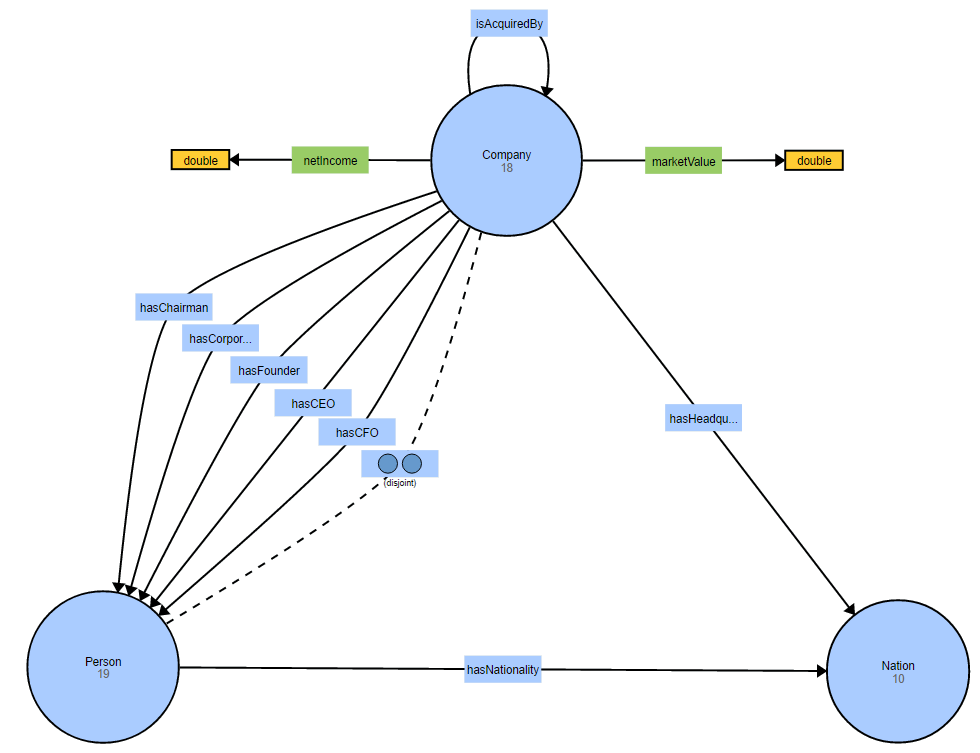
\includegraphics[width=10cm, height=8cm]{fig/ERDiagram.png}
\label{fig:ontology}
    \caption{The ER Diagram.}
\end{figure}


\section{Parsing}
\label{sec:parsing}

The parser is responsible to generate the LTAG/DUDES representation of a question expressed in natural language\footnote{we have restricted our research to the English language.}. 
%
The parser takes in input a natural language sentence $S$, the grammar $G$ and the ontology $O$ \footnote{as stated in the previous sections, we assume that $G$ is aligned to $O$ through a lexicon.}.
%
In particular, it leverages $G$ to recognize lexical entries in $S$, and $O$ to execute reasoning steps for disambiguation during parsing.
%
The generated DUDES is finally used by the applicatio control layer to compose the SPARQL query to be submitted to the ontology.


The parser has been designed addressing two main requirement: \textit{correctness} and \textit{minimization of the syntactic/semantic search space}, which is the most critical aspect to achieve better performance.
%
The previous requirements have been met through a parsing algorithm that is (i) deterministic (ii) greedy and (iii) particularily focused on structural aspects of LTAG.
Furthermore, the performance boost in terms of response-time have been achieved though the minimization of the interaction with the ontology.

The parsing process is carried out by two main functional components: 
(i) the \texttt{Tokenizer}, which recognizes in the sentence textual patterns that can be traced back to grammar entries, and sequentially emit them as tokens, and 
(ii) the \texttt{Parser} itself, which consumes these tokens, composing them to make LTAG/DUDES compositions\footnote{both substitutions and adjunctions.}.

In Section~\ref{sec:parsing-tokenization} and Section~\ref{sec:parsing-algorithm} we describe and motivate the architectural choices and the pseudocode realizing tokenization and the parsing algorithm, respectively.
%
Furthermore, in Section~\ref{sec:parsing-ambiguities} and Section~\ref{sec:parsing-support-dudes-composition} we show how our parser solve ambiguities through reasoning and how it supports DUDES composition though main variables mappings.

\subsection{Tokenization}
\label{sec:parsing-tokenization}

Given a grammar $G$ and a sentence $S$, the tokenization phasepartitions $S$ in a ordered sequence of regular expressions $\{\pi\}$, each one referring at least one elementary LTAG/DUDES in $G$.
%
The \texttt{Tokenizer} is the software component responsible to execute the tokenization pahse.

In Figure~\ref{fig:tokenizer-sample} we show some notable execution of the tokenization phase.
%
Every time the \texttt{Tokenizer} is invoked on $S$ with $G$, it looks in $S$ for the \textit{longest regular expression} matching an entry in $G$.
%
Once the regular expression has been matched, the \texttt{Tokenizer} emits a \textit{token} $t$, that is an element defined as follows:

\begin{equation}
\label{eqn:token}
token:=(regexp,pos,candidates)
\end{equation}

where
$regexp$ is the regular expression matched in the substring of $S$ starting at position $pos$, and
$candidates$ is the list of LTAG/DUDES in $G$ associated with $regexp$.

Notice that $pos$ is recorded inside a token because it can be used by the parsing algorithm to always be able to locate a token inside the sentence.

\begin{figure}[tp]
	\centering
	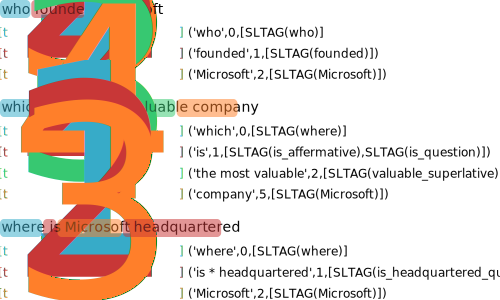
\includegraphics[width=0.8\columnwidth]{./fig/tokenizer-sample}
	\caption{An example of the tokenization phase. In this figure, we denote with \textit{LTAG/DUDES('word')} the elementary LTAG/DUDES associated to the entry \textit{'word'}.}
	\label{fig:tokenizer-sample}
\end{figure}

The \texttt{Tokenizer} is stateful component, hence it leverages convenient data structures to incapsulate its state.
%
The most important one is the \texttt{TokenizerBuffer}, that records whether or not a word in $S$ has been already tokenized.

In Algorithm~\ref{alg:tokenizer} we show the pseudocode of the tokenization process.
%
The \texttt{Tokenizer} exposes a convenient API to iterate over tokens, that is clearly inspired to the well known API provided by Java generic iterators.

\begin{algorithm}[t]
	\SetKwProg{Fn}{Function}{}{}  
	%\Fn{nextTokenizable()}{
	%\For{$b\in buffer$}{
	%	\If{$b.tokenizable\; \& \; b.tokenized$}{
	%		\KwResult{$buffer.index(b)$}
	%	}
	%}
	%\KwResult{$-1$}
	%}	
	
	\Fn{hasNext()}{
	%\KwResult{$nextTokenizable() \neq -1$}
	}
	
	\Fn{next()} {
		$start \leftarrow nextTokenizableIndex()$ \\
		\If{$\neg start1$}{
			\KwResult{$NULL$}
		}
	
		$end \leftarrow start$ \\
		
		\While{$end < buffer.size$}{
			$elem \leftarrow buffer.get(end)$ \\
			\If{$elem.tokenized = False$}{
				$tmpRegexp.concat(elem.word)$ \\
			}
			$matchType \leftarrow grammar.matchMode(tmpRegexp)$ \\
			\If{$matchType = FULL$}{
				$candidates \leftarrow grammar.getAll(tmpRegexp)$ \\
				$regexp \leftarrow tmpRegexp$ \\
				$buffer.get(end).tokenized \leftarrow True$ \\
				\If{$returnFirstFull = True$}{
					break
				}
			}
			\ElseIf{$matchType = NONE$}{
				break
			}
			\ElseIf{$matchType = PART$}{
				$buffer.get(end).tokenized \leftarrow True$ \\
			}
			\ElseIf{$matchType = STAR$}{
				\If{$consuming = False$}{
					$consuming \leftarrow True$ \\
					$startConsuming \leftarrow end$ \\
				}
				\Else{
					\If{$end = buff.size - 1$}{
						$consuming \leftarrow False$ \\
						$end \leftarrow startConsuming - 1$ \\
						$returnFirstFull \leftarrow True$ \\
					}
				}
			}
		
			$end \leftarrow end + 1$ \\
		}
	
		\KwResult{$Token(regexp,pos,candidates)$}		
	}
	\caption{Pseudocode of the \texttt{Tokenizer} API.}
	\label{alg:tokenizer}
\end{algorithm}

Some functions in Algorithm~\ref{alg:tokenizer} have not been formally defined because they are pretty self-explanatory or have been partially introduced in previous sections.
For reader's sake, we briefly describe the most important ones here. 

Recall that an entry $e$ in grammar $G$ is a tuple

\begin{equation}
\label{eqn:grammar-entry}
e:=(regexp,LTAG/DUDES)
\end{equation}

where
$regexp$ is the regular expression representing the syntactic usage of $e$ in a sentence, and
$LTAG/DUDES$ is the elementary LTAG/DUDES in $G$ representing the syntax and semantics of $e$.

\texttt{grammar.matchMode(str)} matches the specified string str against the entries in grammar. 
%
The following matching modes have are defined:
%
\begin{itemize}
	\item[FULL] the grammar contains an entry matching str, and no entry starting with it. 
	For example, the entry \textit{'Microsoft'} matches is such way the grammar $\{who,founded,Microsoft\}$.
	
	\item[PART] the grammar contains no entry matching str, but an entry starting with it.
	For example, the entry \textit{'founders'} matches is such way the grammar $\{who,are,the,founders of,Microsoft\}$.
	
	\item[STAR] the grammar contains no entry matching str, but a entry starting with it and consuming the last part of it with the \textit{star-operator (*)}.
	For example, the entry \textit{'is'} matches is such way the grammar $\{where,is\;*\;headquartered,Microsoft\}$.

	\item[NONE] the grammar contains no entry matching str in one of the previous mode.
	For example, the entry \textit{'Google'} matches is such way the grammar $\{who,founded,Microsoft\}$.
\end{itemize}

\texttt{grammar.getAll(entry)} retrieves from the grammar all the SLTAGs associated with a regular expression matching the entry in \texttt{FULL} mode.
\subsection{Parsing Algorithm}
\label{sec:parsing-algorithm}

The parser we propose adopts an algorithm aiming to reduce the syntactic/semantic search space and response-time of the parsing process.
%
The search space reduction is achieved by the adoption of a greedy approach, consuming tokens left-to-right and eventually buffering ambiguities.
%
The response-time reduction is achieved by the limitation of the interaction with the ontology during the parsing process. 
%
Such a limitation is achieved by limiting the ambiguity resolution process to those candidates that are strictly semantically ambiguous.
%
In fact, all candidates that are infeasible due to their LTAG structure are excluded before the ambiguity resolution step. 

The parser is a stateful component, hence it leverages convenient data structures to encapsulate its state.
%
The parser state is defined as follows:

\begin{equation}
\label{eqn:parser-state}
	\Sigma:=(words,position,main,waitBuff,ambiguityBuff)
\end{equation}

where
\textit{words} is the list of words in the sentence,
\textit{position} is the current parsing position in the sentence,
main it the current working LTAG/DUDES ($S$-rooted),
\textit{waitBuff} is the data structure that buffers LTAG/DUDES that are not ambiguous, but are waiting to be composed with the $main$ and 
\textit{ambiguityBuff} is the data structure that buffer ambiguous LTAG/DUDES.

In Algorithm~\ref{alg:parser} we show the pseudocode of the parsing process.
%
The \texttt{Parser} exposes a very simple API, made up of only one function.

\begin{algorithm}[t]
\label{alg:parser}
\SetKwProg{Fn}{Function}{}{}  

\Fn{parse (grammar,ontology,question)} {
	$state \leftarrow new\; ParserState(question)$ \\
	$tokenizer \leftarrow new\; Tokenizer(grammar,question)$ \\
	
	\While{$token = tokenizer.next()$}{
		$candidates \leftarrow token.candidates$ \\
		\If{$candidates.isEmpty()$}{
			Error(Cannot find suitable LTAG/DUDES for lexical pattern)
		}
		\If{$candidates.size > 1$}{
			filterAmbiguities(state,candidates,ontology)
		}
	
		\If{$candidates.size = 1$}{
			$candidate \leftarrow candidates.get(0)$ \\
			\ElseIf{$isSentence(candidate)$}{
				\If{$\neg state.curr = NULL$}{
					Error(multiple sentence root found) \\
				}
				$state.curr \leftarrow candidate$ \\
			}
			\Else{
				produce(state,candidate)
			}
		}
	
		\If{$\neg state.curr = NULL$}{
			consume(state) \\
		}		
	}

	\If{$state.curr = NULL$}{
		Error(Cannot build LTAG/DUDES)
	}
	
	\For{$ambiguity \in state.ambiguities$}{
		solveAmbiguity(state,ontology,ambiguity) \\
	}

	$state.curr.semantics.isSelect \leftarrow \neg isAskSentence(question)$ \\
	
	\KwResult{$curr$}
}
\caption{Pseudocode of the \texttt{Parser} API.}
\end{algorithm}

Some functions in Algorithm~\ref{alg:parser} have not been formally defined because they are pretty self-explanatory or have been partially introduced in previous sections.
%
For reader's sake, we briefly describe the most important ones here.
%
The function \texttt{isAskSentence(question)} checks if the given \textit{question} should produce an ASK SPARQL query, rather than a SELECT one. It returns true if the question starts with one of the following words: \textit{do,does,did,am,is,are,was,were}.
%
The function \texttt{isSentence(candidate)} checks whether or not the given SLTAG \textit{candidate} has an LTAG rooted in the \textit{S syntax category}.

The function \texttt{filterAmbiguities(state,candidates)} is called when multiple elementary LTAG/DUDES has been found for the given lexical entry.
%
Given the set of candidates, it leverages the current parser state to filter out those that are not feasible due to their LTAG structure.
%
All those candidates that cannot be filtered out in such a way are considered semantically ambiguous and are buffered to be solved later on.

The function \texttt{produce(state,candidate)} adds the given LTAG/DUDES \textit{candidate} to the parser queue. Such a queue is useful to buffer those LTAG/DUDES that cannot be processed until a S-rooted LTAG/DUDES has been found.
%
The function \texttt{consume(state)} consumes the buffered candidates, composing them with the current main LTAG/DUDES. The combination gives an higher priority to candidates for substitution with respect to candidates for adjunctions.

The function \texttt{solveAmbiguity(state,ontology,ambiguity)} solves the remaining semantic ambiguities. In Section~\ref{sec:parsing-ambiguities} we go into details of the ambiguities resolution process.
\subsection{Ambiguities}
\label{sec:parsing-ambiguities}

When a sentence contains a lexical entry that corresponds to multiple elementary LTAG/DUDES in grammar, we say that an \textit{ambiguity} is occurring.
%
A \textit{syntactic ambiguity} occurs when an entry corresponds to multiple elementary LTAG/DUDES with different LTAG
%
A \textit{semantic ambiguity} occures when and entry corresponds to multiple elementary LTAG/DUDES, with same LTAG and different DUDES.
%
Typically, a syntactic ambiguity is easier to solve than a semantic one, because the former can be solved by structural analysis of LTAG, while the latter needs some resoning steps.

In our solution, we solve both form of ambiguities.
%
In particular, when ambiguities arise, the colliding LTAG are structurally analyzed to filter out all syntactic ambiguities.
%
All semantic ambiguities are solved by checking the consistency of their DUDES with respect to the given ontology.

In Figure~\ref{fig:ambiguities-1} and Figure~\ref{fig:ambiguities-2} we give an example of ambiguities resolution.
%
Let us consider the question \textit{'Is Satya Nadella italian?'}. Here we have the following ambiguities:

\begin{itemize}
\item the entry \textit{'is'} induces a syntactic ambiguity because it corresponds to the elementary LTAG/DUDES with LTAG (a) and (b).
%
The ambiguity is solved by excluding (a), because it contains a substitution node on the left of the lexical entry, hence it cannot suitable to parse the first word of a sentence. 
%
Finally, (b) is considered as to be the only feasible LTAG/DUDES.

\item the entry \textit{'italian'} induces a syntactic/semantic ambiguity because it corresponds to the elementary LTAG/DUDES with LTAG (c)/(d) and DUDES (e)/(f).
%
The ambiguity is solved in two steps.
%
First, the LTAGs (d) with DUDES (e) and (f) are excluded because they cannot be adjuncted to the main LTAG/DUDES.
%
Then, (f) is excluded because the proposition \textit{hasHeadquarter(x,y)} cannot have domain \textit{Person} as the entry `Satya Nadella` has.
%
Finally, the LTAG (c) with DUDES (e) is considered as to be the only feasible LTAG/DUDES.
\end{itemize}

\begin{figure}[tp]
\caption{An example of syntactic ambiguity resolution. Ambiguous LTAG for the entry \textit{'is'}.}
\label{fig:ambiguities-1}
	\begin{tabular}{ p{10em} p{10em} }
		\begin{center}
			(a)
			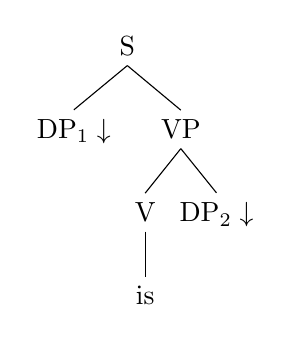
\begin{tikzpicture}
			\Tree [.S [.DP$_1\downarrow$ ] [.VP [.V is ] [.DP$_2\downarrow$ ] ] ]
			\end{tikzpicture}
		\end{center}		
		&
		\begin{center}
			(b)
			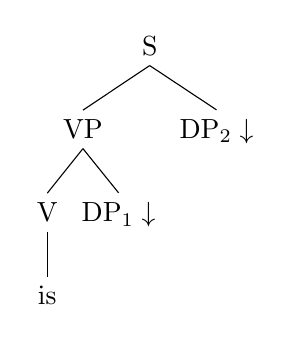
\begin{tikzpicture}
			\Tree [.S [.VP [.V is ] [.DP$_1\downarrow$ ] ] [.DP$_2\downarrow$ ] ]
			\end{tikzpicture}
		\end{center}
	\end{tabular}
\end{figure}

\begin{figure}[tp]
\caption{An example of syntactic/semantic ambiguity resolution. Ambiguous LTAG/DUDES for the entry \textit{'italian'}.}
\label{fig:ambiguities-2}
\begin{tabular}{ p{10em} p{10em} }
	\begin{center}
	(c)
	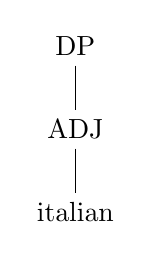
\begin{tikzpicture}
	\Tree [.DP [.ADJ italian ] ]
	\end{tikzpicture}
	\end{center}		
	&
	\begin{center}
	(d)
	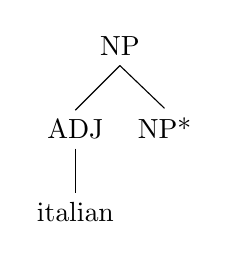
\begin{tikzpicture}
	\Tree [.NP [.ADJ italian ] [.NP* ] ]
	\end{tikzpicture}
	\end{center}		
	\\
	\begin{center}
	(e)
	\begin{tabular}{|c|l|}
		\hline
		\mbox{x} & \\ 
		\hline
		\multicolumn{2}{|l|}{
			$hasNationality(x,y)$
		}\\
		\multicolumn{2}{|l|}{
			$y=Italy$
		}\\
		\hline
		\multicolumn{2}{|l|}{
			\mbox{}
		}\\
		\hline
	\end{tabular}
	\end{center}
	&
	\begin{center}
	(f)
	\begin{tabular}{|c|l|}
		\hline
		\mbox{x} & \\ 
		\hline
		\multicolumn{2}{|l|}{
			$hasHeadquarter(x,y)$
		}\\
		\multicolumn{2}{|l|}{
			$y=Italy$
		}\\
		\hline
		\multicolumn{2}{|l|}{
			\mbox{}
		}\\
		\hline
	\end{tabular}
	\end{center}	
\end{tabular}
\end{figure}

Our parse leverages a reasoning step to solve semantic ambiguities.
%
Whenever a semantic ambiguities arise, a SPARQL query is generated from the DRS statements of each ambiguous DUDES to test its feasibility.

In the following Figures~\ref{fig:ambiguities-resolution-a}-\ref{fig:ambiguities-sparql} we can see an example.
%
Let us consider the main LTAG/DUDES (a) and the ambiguous LTAG/DUDES.
%
The feasibility of DUDES in (b) with respect to (a) is tested by the SPARQL query in Figure~\ref{fig:ambiguities-sparql}. Since the query returns True only for the second DUDES, the first one is excluded.

\begin{figure}[tp]
\caption{An example of ambiguity resolution through reasoning. The main LTAG/DUDES (a)}
\label{fig:ambiguities-resolution-a}
\begin{tabular}{ p{10em} p{10em} }
	\begin{center}
	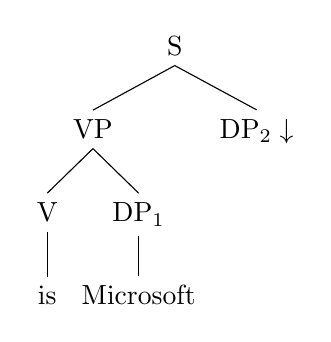
\begin{tikzpicture}
	\Tree [.S [.VP [.V is ] [.DP$_1$ Microsoft ] ] [.DP$_2\downarrow$ ] ]
	\end{tikzpicture}
	\end{center}		
	&
	\begin{center}
	\begin{tabular}{|c|l|}
		\hline
		\mbox{} & x y \\ 
		\hline
		\multicolumn{2}{|l|}{
			$x=Microsoft$
		}\\
		\multicolumn{2}{|l|}{
			$x=y$
		}\\
		\hline
		\multicolumn{2}{|l|}{
			\mbox{$(y,DP_2)$}
		}\\
		\hline
	\end{tabular}
	\end{center}
\end{tabular}
\end{figure}

\begin{figure}[tp]
\caption{An example of ambiguity resolution through reasoning. The LTAG/DUDES that must be checked for semantic feasibility (b)}
\label{fig:ambiguities-resolution-b}
\begin{tabular}{ p{10em} p{10em} p{10em} }
	\begin{center}
	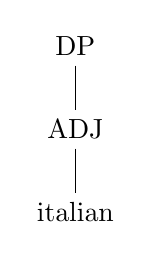
\begin{tikzpicture}
	\Tree [.DP [.ADJ italian ] ]	
	\end{tikzpicture}
	\end{center}		
	&
	\begin{center}
	\begin{tabular}{|c|l|}
		\hline
		\mbox{x} & x y \\ 
		\hline
		\multicolumn{2}{|l|}{
			$hasNationality(x,y)$
		}\\
		\multicolumn{2}{|l|}{
			$y=Italy$
		}\\
		\hline
		\multicolumn{2}{|l|}{
			\mbox{}
		} \\
		\hline
	\end{tabular}
	\end{center}
	&
	\begin{center}
	\begin{tabular}{|c|l|}
		\hline
		\mbox{x} & x y \\ 
		\hline
		\multicolumn{2}{|l|}{
			$hasHeadquarter(x,y)$
		}\\
		\multicolumn{2}{|l|}{
			$y=Italy$
		}\\
		\hline
		\multicolumn{2}{|l|}{
			\mbox{}
		} \\
		\hline
	\end{tabular}
	\end{center}	
\end{tabular}
\end{figure}

\begin{figure}[tp]
\caption{An example of ambiguity resolution though reasoning. The SPARQL query to test semantic feasibility for ambiguity in Figure~\ref{fig:ambiguities-resolution-b}.}
\label{fig:ambiguities-sparql}
\begin{center}
\begin{verbatim}
ASK WHERE {
    :Microsoft rdf:type ?class1 . 
    :Italy rdf:type ?class2 . 
    hasNationality rdfs:domain ?class1 . 
    hasNationality rdfs:range ?class2
} 
\end{verbatim}	
\end{center}
\end{figure}
\subsection{Support to DUDES composition}
\label{sec:parsing-support-dudes-composition}

In this section we show how our parser supports DUDES composition though \textit{main variable mappings}.
%
First of all, we state here some useful definitions.
%
An \textit{obfuscated variable} is a main variable of a DUDES that is lost at time $t_{1}$ due to substitution, though it should be referenced by some other DUDES at time $t_{2}>t_{1}$.
%
We call \textit{obfuscating substitution} a DUDES substitution that creates an obfuscating variable.

In Figure~\ref{fig:obfuscating-substitution-1} we show an example of obfuscating substitution. 
%
Let us consider the question \textit{'did Microsoft acquire an italian company?'}.
%
We have the main LTAG/DUDES (a), the waiting LTAG/DUDES (b) and the ambiguous LTAG/DUDES (c).
%
The substitution of (b) in (a) is an obfuscating substitution, because once executed, the resulting main LTAG/DUDES in Figure~\ref{fig:obfuscating-substitution-2}.
%
Notice that the resulting main LTAG/DUDES does not have the main variable any more, due to the normal DUDES substitution.
%
Such a situation makes the adjunction of (c) loose its semantic value, due to the absence of the main variable.

Our parser overcome this limitation by detecting obfuscating substitutions. 
%
In particular, it records obfuscated variable, making them accessible by successive adjunctions.
%
In this way, the semantic value of (c) would have never been lost.
%
When (c) is processed, the parser detects that it is looking for an obfuscated variable and makes it temporaly available in the semantics of the main LTAG/DUDES.
%
Once the obfuscated variable have been used, it will never be considered any more.

\begin{figure}[H]
	\caption{An example of obfuscating substitution (a),(b),(c).}
	\label{fig:obfuscating-substitution-1}
	\begin{tabular}{ p{10em} p{10em} p{10em} }
		\begin{center}
		(a)
		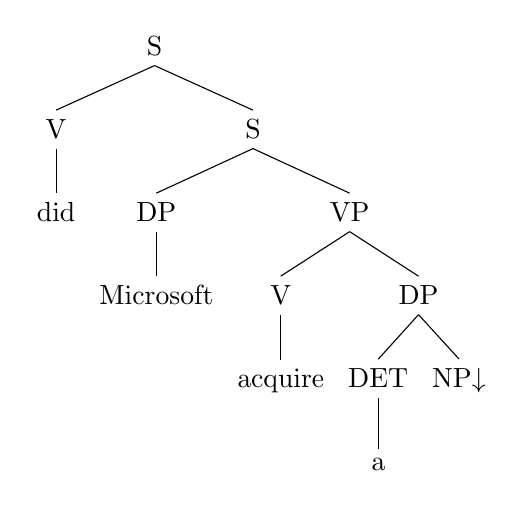
\begin{tikzpicture}
			\Tree [.S [.V did ] [.S [.DP  Microsoft ] [.VP [.V acquire ] [.DP [.DET a ] [.NP$\downarrow$ ] ] ] ] ]
		\end{tikzpicture}
		\end{center}		
		&
		\begin{center}
		(b)
		
\begin{tikzpicture}
			\Tree [.NP company ]	
		\end{tikzpicture}
		\end{center}		
		&
		\begin{center}
		(c)
		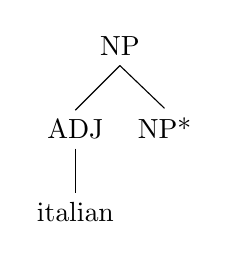
\begin{tikzpicture}
			\Tree [.NP [.ADJ italian ] [.NP* ] ]
		\end{tikzpicture}
		\end{center}		
		
		\\
			
		\begin{center}
		\begin{tabular}{|c|l|}
		\hline
		\mbox{} & x y \\ 
		\hline
		\multicolumn{2}{|l|}{
			$isAcquiredBy(x,y)$
		}\\
		\multicolumn{2}{|l|}{
			$y=Microsoft$
		}\\
		\hline
		\multicolumn{2}{|l|}{
			\mbox{$(x,NP)$}
		} \\
		\hline
		\end{tabular}
		\end{center}
		&
		\begin{center}
		\begin{tabular}{|c|l|}
		\hline
		\mbox{x} & x \\ 
		\hline
		\multicolumn{2}{|l|}{
			$Company(x)$
		}\\
		\hline
		\multicolumn{2}{|l|}{
			\mbox{}
		} \\
		\hline
		\end{tabular}
		\end{center}	
		&
		\begin{center}
		\begin{tabular}{|c|l|}
		\hline
		\mbox{x} & x y \\ 
		\hline
		\multicolumn{2}{|l|}{
			$hasHeadquarter(x,y)$
		}\\
		\multicolumn{2}{|l|}{
			$y=Italy$
		}\\
		\hline
		\multicolumn{2}{|l|}{
			\mbox{}
		} \\
		\hline
		\end{tabular}
		\end{center}
	\end{tabular}
\end{figure}

\begin{figure}[H]
	\caption{An example of obfuscating substitution. The substitution obfuscates the main variable.}
	\label{fig:obfuscating-substitution-2}
	\begin{tabular}{ p{10em} p{10em} }
		\begin{center}
		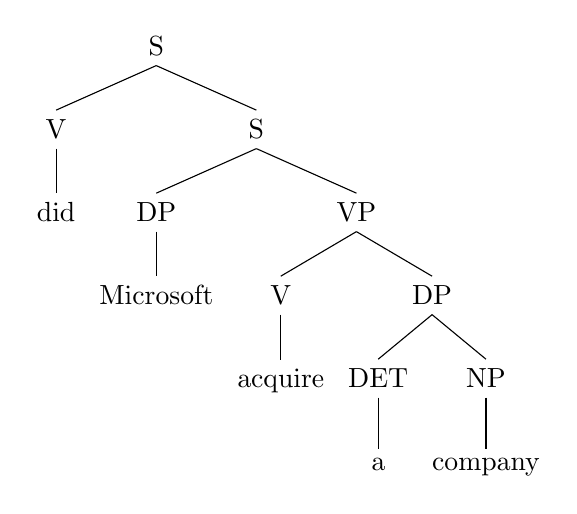
\begin{tikzpicture}
		\Tree [.S [.V did ] [.S [.DP  Microsoft ] [.VP [.V acquire ] [.DP [.DET a ] [.NP company ] ] ] ] ]
		\end{tikzpicture}
		\end{center}
		\begin{center}
		\begin{tabular}{|c|l|}
			\hline
			\mbox{} & x y \\ 
			\hline
			\multicolumn{2}{|l|}{
				$isAcquiredBy(x,y)$
			}\\
			\multicolumn{2}{|l|}{
				$y=Microsoft$
			}\\	
			\multicolumn{2}{|l|}{
				$Company(x)$
			}\\			
			\hline
			\multicolumn{2}{|l|}{
				\mbox{}
			} \\
			\hline
		\end{tabular}
		\end{center}	
	\end{tabular}
\end{figure}

\begin{figure}[tp]
	\caption{An example of obfuscating substitution. The obfuscated variable is not accessible for the adjunction, causing the main variabl refence to be lost.}
	\label{fig:obfuscating-substitution-3}
	\begin{tabular}{ p{10em} }
		\begin{center}
		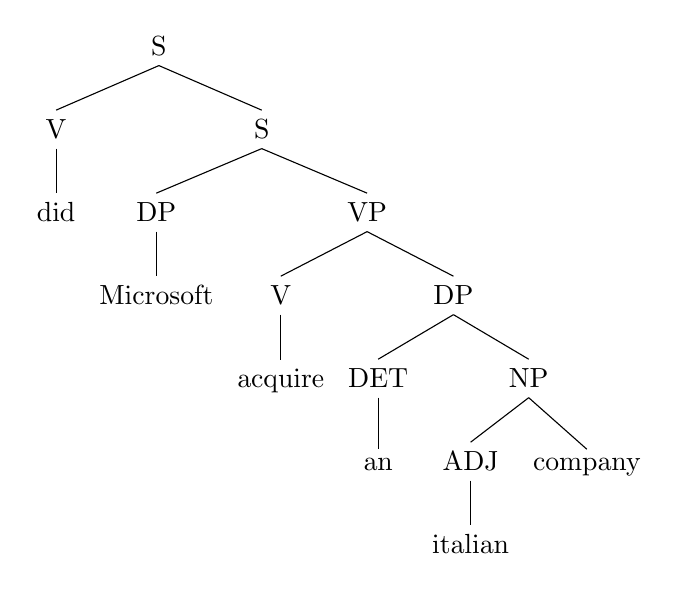
\begin{tikzpicture}
			\Tree [.S [.V did ] [.S [.DP  Microsoft ] [.VP [.V acquire ] [.DP [.DET an ] [.NP [.ADJ italian ] company ] ] ] ] ]
		\end{tikzpicture}
		\end{center}	
		\\
		\begin{center}
			\begin{tabular}{|c|l|}
				\hline
				\mbox{} & x y z\\ 
				\hline
				\multicolumn{2}{|l|}{
					$isAcquiredBy(x,y)$
				}\\
				\multicolumn{2}{|l|}{
					$y=Microsoft$
				}\\
				\multicolumn{2}{|l|}{
					$Company(x)$
				}\\
				\multicolumn{2}{|l|}{
					$hasHeadquarter(z,t)$
				}\\
				\multicolumn{2}{|l|}{
					$t=Italy$
				}\\
				\hline
				\multicolumn{2}{|l|}{
					\mbox{}
				} \\
				\hline
			\end{tabular}
		\end{center}	
	\end{tabular}
\end{figure}

\section{Implementation}
\label{sec:implementation}
% ALL

Ontoqa has been realized as a Java\footnote{Oracle Java SE 8} web and standalone application, packaged with Maven.
%
Ontoqa can be executed both as a standalone application and as a web application.
%
All functionalities has been tested carefully against 224 total unit tests.

Ontoqa leverages some well known technologies. Here we present them, giving an idea about how they have been used in our implementation. The reader may refer to the open source code of the project and the corresponding Javadocs to get into the implementation details.


\begin{itemize}
	\item[Ontology] INSERT HERE
	
	\item[Lexicon] The lexical information about ontology is reported in Java by using the APIs provided by the "Semantic Computing Group @ Bielefeld University". The APIs allow the representation of the lemon model in java and the use of lexinfo for generating grammar. The library was manipulated to shape the following lemon properties: 
	\begin{itemize}
		\item Recognition of entries of composite words
		\item Tense and number of different forms of entry 
	\end{itemize}	
Finally, where necessary, a parsing of meaningful terms extracted from paths has been implemented.
The library provided has been to retrieve the ontology represented by the Lemon model from the RDF file and to get a list of Lexical Entry consisting of the most relevant properties shown in the figure:
\begin{figure}[tp]
   \centering
    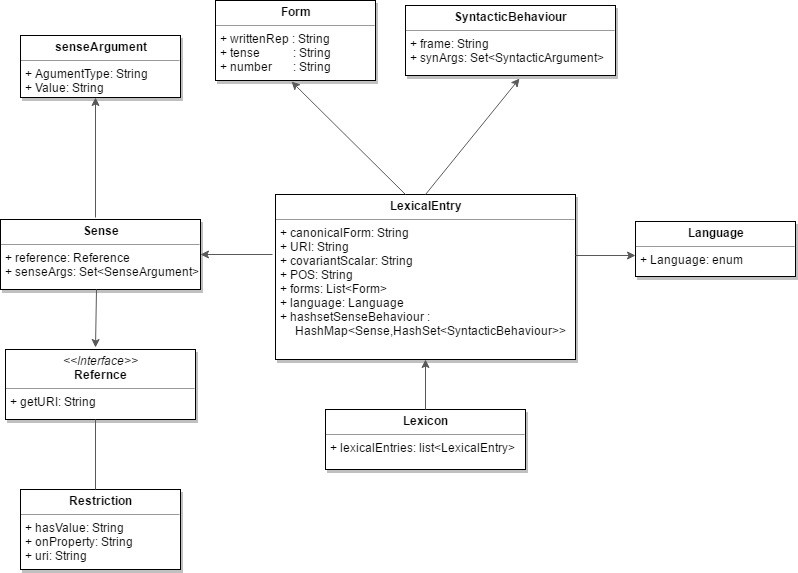
\includegraphics[scale=100]{./fig/lemon}
    \label{fig: lemon}
\end{figure}

	\item[I/O] we used the Jackson core library and data-binding modules to implement data representation in JSON and YAML format.
	
	\item[CLI] we used Apache CLI to implement options and argument parsing for the command line interface.
	
	\item[Web UI] we used AngularJS, JQuery and JavaScript for navigation logic and HTML5 and Bootstrap for the page style.
	
	\item[Web Service] we used Spring Framework and Spring MVC to implement the REST service interface.
	
	\item[Logging] we used SLF4J to implement logging ayer as facade, and Logback as the underlying logging framework.
	
	\item[Development] we used Lombok to implement bean constructors, getter/setters, thus minimizing code redundancy.
	
	\item[Testing] we used JUnit4 to implement unit testing suites.
\end{itemize}


\section{Sample execution}
\label{sec:sample-execution}
% DEBORA
In this section we will see some sample execution from natural language to the final answer. Let's start with a simple example:

\begin{enumerate}
\item "\textit{Who is the chief financial officer of Apple?}"
As we can see from the \textit{Fig.2} in the Section \ref{sec:architecture}, our input is an english natural language question.  The parsing algorithm described in section \ref{sec:parsing}, gives us a LTAG. Next, syntactic and semantic composition rules apply in tandem in order to construct a LTAG and a DUDES:
\begin{itemize}
\item \textbf{LTAG}
\medskip
\begin{center}
\begin{tabular}{ p{10em} p{10em} p{10em} }
	\label{tbl:grammar.example1}
	\begin{center}{(1)} \end{center}
	\begin{center}
		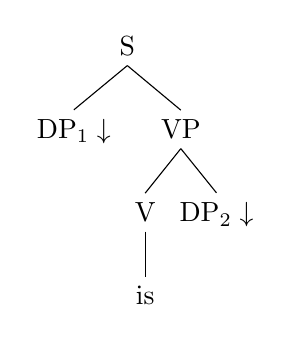
\begin{tikzpicture}
		\Tree [.S [.DP$_1\downarrow$ ] [.VP [.V is ] DP$_2\downarrow$ ] ]	
		\end{tikzpicture}
	\end{center}

	&
	
	\begin{center}{(2)} \end{center}
	\begin{center}
		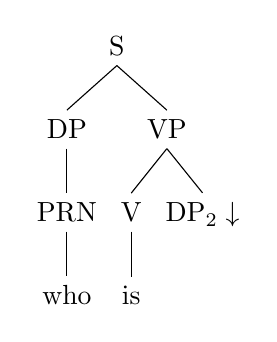
\begin{tikzpicture}
		\Tree [.S [.DP  [.PRN who ] ] [.VP [.V is ] DP$_2\downarrow$ ] ]	
		\end{tikzpicture}
	\end{center}
	
	&
	
	\begin{center}{(3)} \end{center}
	\begin{center}
		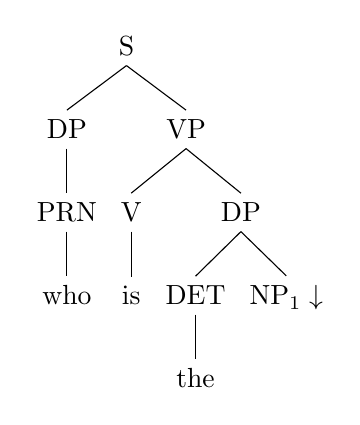
\begin{tikzpicture}
		\Tree [.S [.DP  [.PRN who ] ] [.VP [.V is ] [.DP  [.DET the ] [.NP$_1\downarrow$ ]] ] ]	
		\end{tikzpicture}
	\end{center}
	\\
\end{tabular}
\end{center}
\medskip

\medskip
\begin{center}
\begin{tabular}{ p{10em} p{10em} p{10em} p{10em} }
	\label{tbl:grammar.example1}
		
	\begin{center}{(4)} \end{center}
	\begin{center}
		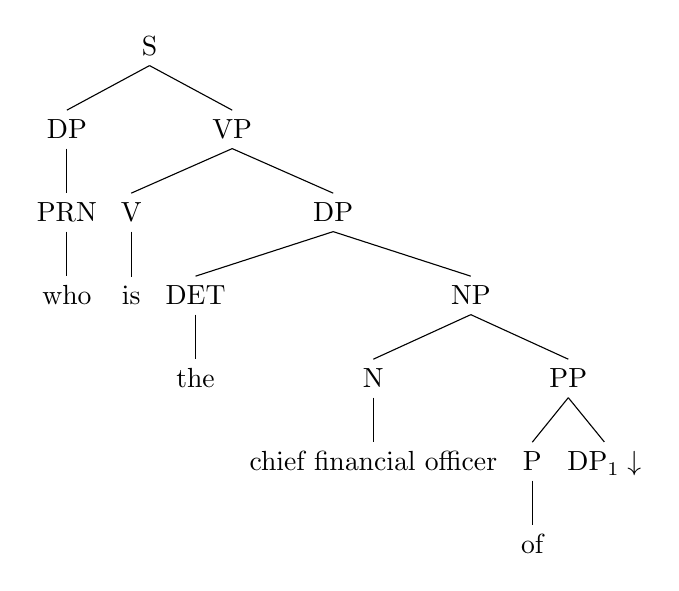
\begin{tikzpicture}
		\Tree [.S [.DP  [.PRN who ] ] [.VP [.V is ] [.DP  [.DET the ] [.NP [.N \text{chief financial officer} ] [.PP [.P of ] DP$_1\downarrow$ ]]
] ] ]	
		\end{tikzpicture}
	\end{center}
	
	&
	\mbox{}
	&
	\begin{center}{(5)} \end{center}
	\begin{center}
	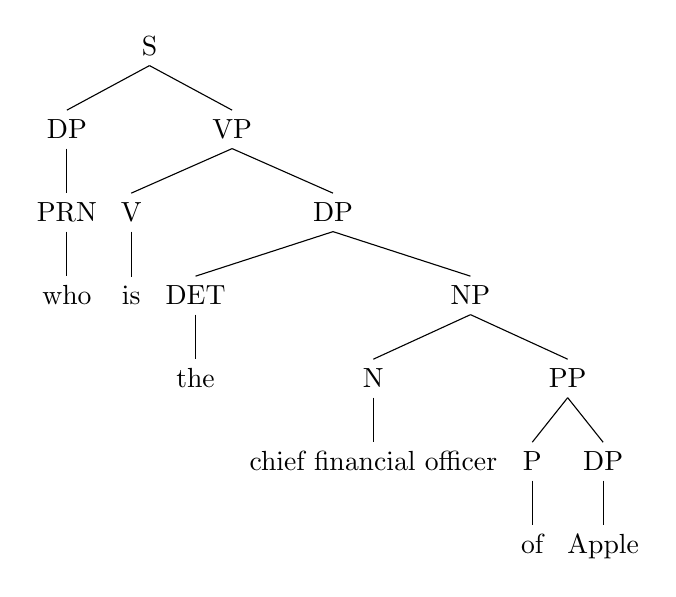
\begin{tikzpicture}
	\Tree [.S [.DP  [.PRN who ] ] [.VP [.V is ] [.DP  [.DET the ] [.NP [.N \text{chief financial officer} ] [.PP [.P of ] [.DP Apple ] ]]
] ] ]	
		\end{tikzpicture}
	\end{center}
	&
\mbox{}
	\\
\end{tabular}
\end{center}



\medskip

\item \textbf{DUDES} 
\medskip
\begin{center}
\begin{tabular}{ p{10em} }
	\label{tbl:grammar.example1}
	
	\begin{center}
		\begin{tabular}{|c|l|}
			\hline
			\mbox{} & ?x \\ 
			\hline
			\multicolumn{2}{|l|}{
				$hasCFO(y,x)$
			}\\
			\multicolumn{2}{|l|}{
			$y=Apple$
			}\\
			\hline
			\multicolumn{2}{|l|}{
				\mbox{}
			} \\
			\hline
		\end{tabular}
	\end{center}	
	\\
\end{tabular}
\end{center}
\medskip

\end{itemize}
The final step consists in translating this DUDES into a SPARQL query. Here the query generated by this question:
\\
\\
\textit{PREFIX org: $<http://www.semanticweb.org/organization \# >$}
\\
\\
\textit{SELECT DISTINCT ?x \\
\mbox{}\qquad WHERE $\{$ org:Apple org:hasCFO ?x $\}$}
\\

\item "\textit{What is the most valuable company?}"
A special case is the quantifier \textit{the most}. The process for getting the answer is the same of the prevoius example and the construction of the LTAG is very similar. The particularity of this question is in the semantic representation.
 
\begin{itemize}
\item \textbf{LTAG}
\medskip
\begin{center}
\begin{tabular}{ p{10em} p{10em} p{10em} }
	\label{tbl:grammar.example2}
		
	\mbox{}
	&
	
	\begin{center}
		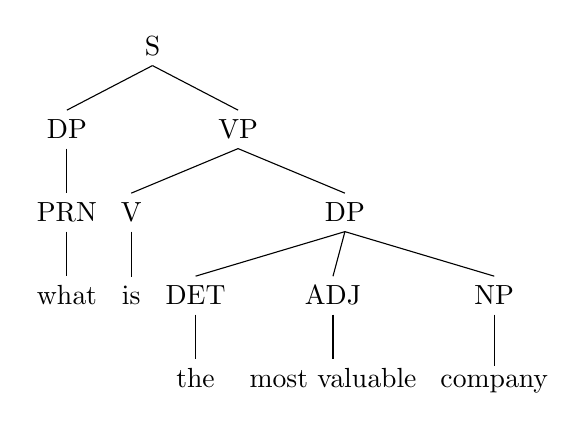
\begin{tikzpicture}
		\Tree [.S [.DP  [.PRN what ] ] [.VP [.V is ] [.DP  [.DET the ] [.ADJ \text{most valuable} ] [.NP company ]] ] ]	
		\end{tikzpicture}
	\end{center}
		
	&
	
	\mbox{}
	
	\\
\end{tabular}
\end{center}
\medskip

\item \textbf{DUDES}	
\medskip
\begin{center}
\begin{tabular}{ p{10em} }
	\label{tbl:grammar.example1}
	
	\begin{center}
		\begin{tabular}{|c|l|}
			\hline
			\mbox{} & ?x \\ 
			\hline
			\multicolumn{2}{|l|}{
				$marketValue(x,y)$
			}\\
			\multicolumn{2}{|l|}{
				$Company(y)$
			}\\
			\multicolumn{2}{|l|}{
				$MAX(x,y)$
			}\\
			\hline
			\multicolumn{2}{|l|}{
				\mbox{}
			} \\
			\hline
		\end{tabular}
	\end{center}	
	\\
\end{tabular}
\end{center}
\medskip
\end{itemize}
The final translation from DUDES generates the following query:
\\
\\
\textit{PREFIX org: $<http://www.semanticweb.org/organization \# >$}
\\
\\
\textit{SELECT DISTINCT ?x \\
\mbox{}\qquad WHERE $\{$ org:x org:marketValue ?y $\}$\\
\mbox{}\qquad ORDER BY DESC(?y)\\
\mbox{}\qquad OFFSET 0\\
\mbox{}\qquad LIMIT 1}\\
\\



		



\item "\textit{Did Microsoft acquire a company headquartered in Italy?}"
The reader can see the use of the adjunction operation in this example. Below the LTAG, the DUDES and the final SPARQL query:
\begin{itemize}
\item \textbf{LTAG}
\medskip
\begin{center}
\begin{tabular}{ p{10em} p{3em} p{10em} p{3em} p{10em} }
	\label{tbl:grammar.example1}
	\begin{center}{(1)} \end{center}
	\begin{center}
		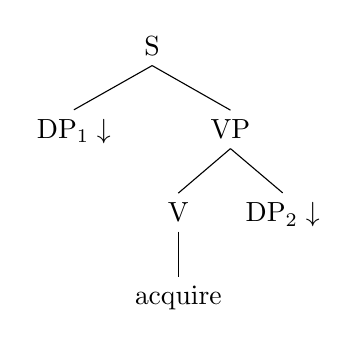
\begin{tikzpicture}
		\Tree [.S [.DP$_1\downarrow$ ] [.VP [.V acquire ] DP$_2\downarrow$ ] ]	
		\end{tikzpicture}
	\end{center}
	
	&
	\mbox{}
	&

	\begin{center}{(2)} \end{center}
	\begin{center}
		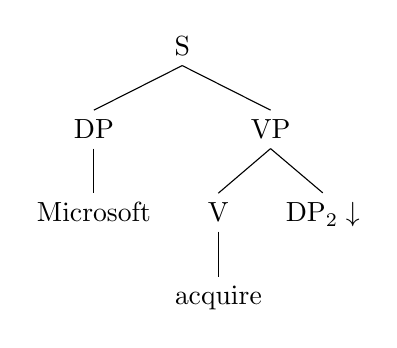
\begin{tikzpicture}
		\Tree [.S [.DP  Microsoft ] [.VP [.V acquire ] DP$_2\downarrow$ ] ]	
		\end{tikzpicture}
	\end{center}
	
	&
	\mbox{}
	&
	
	\begin{center}{(3)} \end{center}
	\begin{center}
		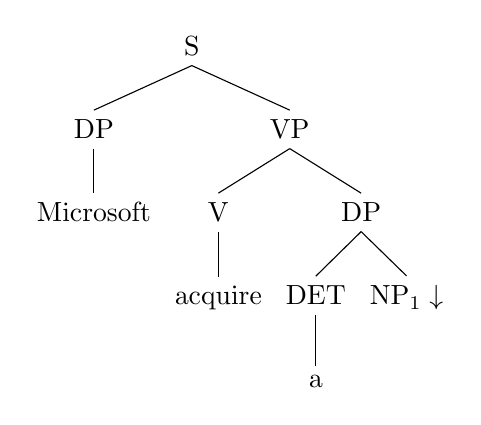
\begin{tikzpicture}
		\Tree [.S [.DP  Microsoft ] [.VP [.V acquire ] [.DP  [.DET a ] [.NP$_1\downarrow$ ]] ] ]	
		\end{tikzpicture}
	\end{center}
	\\
\end{tabular}
\end{center}
\medskip

\medskip
\begin{center}
\begin{tabular}{ p{10em} p{3em} p{10em} p{10em}}
	\label{tbl:grammar.example3}
	\begin{center}{(4)} \end{center}
	\begin{center}
		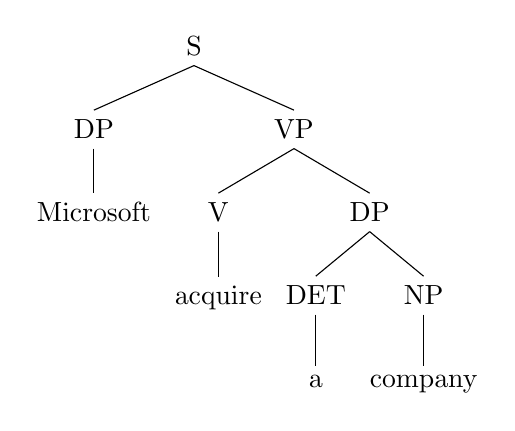
\begin{tikzpicture}
		\Tree [.S [.DP  Microsoft ] [.VP [.V acquire ] [.DP  [.DET a ] [.NP company ]] ] ]	
		\end{tikzpicture}
	\end{center}
	
	&
	\mbox{}
	&

	\begin{center}{(5)} \end{center}
	\begin{center}
		\begin{tikzpicture}
		\Tree [.S [.DP  Microsoft ] [.VP [.V acquire ] [.DP  [.DET a ] [.NP [ company ] [.ADJPP [.ADJ headquartered ] [.PP [.P in ] DP$_1\downarrow$ ] ]]] ] ]	
		\end{tikzpicture}
	\end{center}
	&
	\mbox{}
	\\
\end{tabular}
\end{center}
\medskip

\medskip
\begin{center}
\begin{tabular}{ p{10em} p{6em} p{10em} p{17em}}
	\label{tbl:grammar.example3}
	
	\begin{center}{(6)} \end{center}
	\begin{center}
		\begin{tikzpicture}
		\Tree [.S [.DP  Microsoft ] [.VP [.V acquire ] [.DP  [.DET a ] [.NP [ company ] [.ADJPP [.ADJ headquartered ] [.PP [.P in ] [.DP Italy ] ] ]]] ] ]	
		\end{tikzpicture}
	\end{center}
	
	&
	\mbox{}
	&
	
	\begin{center}{(7)} \end{center}
	\begin{center}
		\begin{tikzpicture}
		\Tree [.S [.V did ] [.DP  Microsoft ] [.VP [.V acquire ] [.DP  [.DET a ] [.NP [ company ] [.ADJPP [.ADJ headquartered ] [.PP [.P in ] [.DP Italy ] ] ]]] ] ]	
		\end{tikzpicture}
	\end{center}
	&
	\mbox{}
	\\
\end{tabular}
\end{center}
\medskip

\item \textbf{DUDES}
\medskip
\begin{center}
\begin{tabular}{ p{10em} }
	\label{tbl:grammar.example3}
	
	\begin{center}
		\begin{tabular}{|c|l|}
			\hline
			\mbox{} & x \\ 
			\hline
			\multicolumn{2}{|l|}{
			$isAcquiredBy(x,y)$
			}\\
			\multicolumn{2}{|l|}{
			$Company(x)$
			}\\
			\multicolumn{2}{|l|}{
			$y=Microsoft$
			}\\
			\multicolumn{2}{|l|}{
			$hasHeadquarter(x,z)$
			}\\
			\multicolumn{2}{|l|}{
			$z=Italy$
			}\\
			\hline
			\multicolumn{2}{|l|}{
				\mbox{}
			} \\
			\hline
		\end{tabular}
	\end{center}	
	\\
\end{tabular}
\end{center}
\medskip
\end{itemize}
The generated query SPARQL is:
\\
\\
\textit{PREFIX org: $<http://www.semanticweb.org/organization \# >$}
\\
\\
\textit{ASK \\
\mbox{}\qquad WHERE $\{$ ?x org:isAcquiredBy org:Microsoft .\\
\mbox{}\qquad \qquad \qquad ?x org:hasHeadquarter org:Italy
\mbox{}\qquad $\}$ \\
\mbox{}\qquad ORDER BY DESC(?y)\\
\mbox{}\qquad OFFSET 0\\
\mbox{}\qquad LIMIT 1}\\
\\ 

\end{enumerate}
\section{Evaluation}
\label{sec:evaluation}

\lipsum[1]
\section{Further Improvements}
\label{sec:improvements}

A possible improvement could be to extend the library provided by the "Semantic Computing Group @ Bielefeld University" as it does not completely cover the properties of Lemon and Lexinfo, but only the most common properties. 

The second improvement concerns ontology, in particular the redefinition of class hierarchy and the extension of domain knowledge.
\section{Conclusions}
\label{sec:conclusions}

In this work we described Ontoqa, a Q\&A web and standalone application which aims to adapt easily to distinct ontologies and lexicons.
%
The proposed solution leverages ontology-driven NLP through the use of the LTAG/DUDES model and a greedy parsing algorithm aiming to reduce both the syntactic and semantic search space.
%
%
% RESULTS
The experimental results show that our system can answer the benchmark questions, with good performance with respect to both response-time.
%
%
% CONCLUSIONS
Our work shows that ontology alignment through the LTAG/DUDES model permits 
high modularization and generalization of the NLP process.
%
Furthermore, such a model suits well to the design of parsing algorithms that can effectively minimize both the syntactic and semantic search space.


%*******************************************************************************
% Bibliography
%*******************************************************************************
\bibliographystyle{acmreferences}
\bibliography{ref/biblio}

\end{document}
